\documentclass [11pt,a4paper]{article}
\usepackage[utf8]{inputenc}
\usepackage[T1]{fontenc}
\usepackage[english]{babel}
\usepackage{textcomp}
\usepackage{lmodern}

% Text Indentation
\usepackage{indentfirst}
\setlength{\parindent}{1cm}

% Section, Subsection & Subsubsection Indentation
\newcommand{\mysection}[1]{
	\setlength{\leftskip}{0cm}
	\section{#1}}
\newcommand{\mysubsection}[1]{
	\setlength{\leftskip}{0.5cm}
	\subsection{#1}}
\newcommand{\mysubsubsection}[1]{
	\setlength{\leftskip}{1cm}
	\subsubsection{#1}}

% Defined header and footer style
\usepackage{fancyhdr}
\pagestyle{fancy}
\renewcommand{\sectionmark}[1]{%
	\markright{\thesection\ #1}}
\fancyhf{}
\fancyhead[LE,RO]{\bfseries\thepage}
\fancyhead[LO]{\bfseries\rightmark}
\fancyhead[RE]{\bfseries\leftmark}
\lfoot{\textcolor{Gray}{\small{Copyright © 2019 Kostandin Caushi, Raffaele Bongo – All rights reserved}}}
\renewcommand{\headrulewidth}{1pt}
\fancyhfoffset[lf]{0mm}

% Page margins, header and footer positions
\usepackage{geometry}
\geometry{
	a4paper,
	total={210mm,297mm},
	left=25mm,
	right=25mm,
	top=35mm,
	bottom=25mm,
	headsep=10mm
	}

\interfootnotelinepenalty=10000

% Tables
\usepackage{tabu}
\usepackage{tabularx}
\usepackage{multirow}
\usepackage{ltablex}
\usepackage{longtable}
\usepackage{float} % To allow the use of H modifier in long tables

% Graphics
\usepackage{graphicx}
\usepackage[dvipsnames, table]{xcolor}

\usepackage{ifthen}
\usepackage{xspace}
\usepackage{enumitem}
\usepackage{amssymb}
\usepackage[pdftex, colorlinks]{hyperref}
\hypersetup{%
	colorlinks = true,
	linkcolor  = black,
	pdfauthor  = {Kostandin Caushi, Raffaele Bongo},
	pdftitle   = {EasyLib}
}
\newcommand{\comment}[1]{{\color{Blue}$\blacktriangleright$ Comment: #1 $\blacktriangleleft$}}

% Java Package
\usepackage{listings}
\usepackage{color}

\definecolor{mygreen}{rgb}{0,0.6,0}
\definecolor{mygray}{rgb}{0.5,0.5,0.5}
\definecolor{mymauve}{rgb}{0.58,0,0.82}

\lstset{ %
	backgroundcolor=\color{white},   % choose the background color; you must add \usepackage{color} or \usepackage{xcolor}; should come as last argument
	basicstyle=\footnotesize,        % the size of the fonts that are used for the code
	breakatwhitespace=false,         % sets if automatic breaks should only happen at whitespace
	breaklines=true,                 % sets automatic line breaking
	captionpos=b,                    % sets the caption-position to bottom
	commentstyle=\color{mygreen},    % comment style
	deletekeywords={...},            % if you want to delete keywords from the given language
	escapeinside={\%*}{*)},          % if you want to add LaTeX within your code
	extendedchars=true,              % lets you use non-ASCII characters; for 8-bits encodings only, does not work with UTF-8
	frame=single,	                   % adds a frame around the code
	keepspaces=true,                 % keeps spaces in text, useful for keeping indentation of code (possibly needs columns=flexible)
	keywordstyle=\color{blue},       % keyword style
	language=Octave,                 % the language of the code
	morekeywords={*,...},            % if you want to add more keywords to the set
	numbers=left,                    % where to put the line-numbers; possible values are (none, left, right)
	numbersep=5pt,                   % how far the line-numbers are from the code
	numberstyle=\tiny\color{mygray}, % the style that is used for the line-numbers
	rulecolor=\color{black},         % if not set, the frame-color may be changed on line-breaks within not-black text (e.g. comments (green here))
	showspaces=false,                % show spaces everywhere adding particular underscores; it overrides 'showstringspaces'
	showstringspaces=false,          % underline spaces within strings only
	showtabs=false,                  % show tabs within strings adding particular underscores
	stepnumber=2,                    % the step between two line-numbers. If it's 1, each line will be numbered
	stringstyle=\color{mymauve},     % string literal style
	tabsize=2,	                   % sets default tabsize to 2 spaces
	title=\lstname                   % show the filename of files included with \lstinputlisting; also try caption instead of title
}

\begin{document}
	\begin{titlepage}
		\centering
		%LOGO
		\begin{figure}
			\vspace*{0mm}
			\centering
			
\includegraphics[scale=0.3]{Images/EasyLib_Logo}
			\\[2cm]
		\end{figure}
		\vspace{5mm}
		\textcolor{Blue}{\textbf{\huge EASYLIB}}\\[15mm]
		\textcolor{Blue}{\textbf{\huge DD}}\\[4mm]
		{\textcolor{Blue}{\textbf{\Large{Design Document}}}}\\
		\vspace{30mm}
		\textit{\large Kostandin Caushi 898749}\\[3mm]
		\textit{\large Raffaele Bongo 900090}\\[3mm]
		\vspace*{30mm}
		Date 12/02/2019\\[1cm]
		\begin{figure}[h]
			\begin{flushright}
				
\includegraphics[scale=0.13]{Images/Polimi_Logo}
			\end{flushright}
		\end{figure}
	\end{titlepage}

%------------------------------
	\begin{center}
	\vspace*{-5mm}
	\renewcommand{\contentsname}{Table of Contents}
	\tableofcontents
	\newpage
	\listoffigures
	\newpage
    \end{center}
	
%-----------------------------
	\ttfamily
	\setlength{\emergencystretch}{45pt}
	\vspace*{-5mm}
\mysection{Introduction}

\mysubsection{Purpose}
The purpose of this document is to provide a full description of the design of the
EasyLib and EasyLib - Librarian mobile applications, two native Android applications, providing insights into the the goal of the system, the design of each component and how the project has been managed.

\mysubsection{Scope}
EasyLib is a mobile application that manage to make easier multiple management tasks that nowadays a library needs to deal with. It answers all the questions for which a library visitor usually stuck for an answer such as books description and availability, waiting queue for reserve a book, events taking place and news related to the library, and make really easy to the book search and reservation. The application allow the user to interface with all the libraries that choose to use EasyLib as management system, using a single identification process to interact with all of them.
EasyLib has been thought to cover also the Librarian necessity and help him into his daily work automatizing the book delivering and returning process and helping him to schedule his work. However, the librarian system that we are going to present in this document is a prototype with a fraction of the functionalities that have been designed and are left to a future upgraded of the app.


\mysubsection{Definitions}
\begin{itemize}
	\item \emph{System :} with the term system we will consider the client-side android applications and the server (not the DB).
\end{itemize}

\mysubsection{Acronyms}
\begin{itemize}
	\setlength{\leftskip}{0.5cm}
	\item \emph{API :} Application Programming Interface
	\item \emph{DB :} Database
\end{itemize}

\mysubsection{Abbreviations}
\begin{itemize}
	\setlength{\leftskip}{0.5cm}
	\item \lbrack Gn] : Goal n
	\item \lbrack Rn] : Requirement n
\end{itemize}

\mysubsection{Document Structure}
This paper is divided in six chapter.\\

The first chapter is composed by an introduction of the system, its application domain, its goals and a glossary containing the most common expression used in order to give to the reader a basic knowledge of the system and to make him understand better the subsequent parts.\\\\
In the second chapter we have provided a list of all the applications goals and the related requirements and we also listed their core functionalities with a synthetic description.\\

The third chapter is devoted to the exposure of the overall design architecture of the system, the identification and definition of all the software components that characterize our system end to end and the external services and libraries used to accomplish all the goals that we aimed to satisfy. We also shown a deployment proposal and non-functionals requirements that we need to respect.\\

The fourth chapter is exploited to show the most relevant decisions taken in the UI design and to show how the application looks to the final user using images taken during the real usage.\\

In the fifth chapter we showed some runtime view diagrams to explain how the most sensitive functionalities of the system are carried out and the interaction between the different hardware tiers and software components.\\

Finally, in the sixth chapter we have put in writing the implementation strategy that we followed to implement the system, how our team has been structured, the implementation process carried on and the test cases performed. 
	
	
	

	\newpage
	\vspace*{-5mm}
\mysection{Overall Description}

\mysubsection{Goals \& Requirements}
\vspace{0.2cm}
\mysubsubsection{EasyLib}
\vspace{0.5cm}
\noindent
\emph{\textbf{[G$_{1}$] : Allow the user to register and login into the system (also throughout external services)}}
\begin{itemize}
	\setlength{\leftskip}{0.5cm}
	\item \lbrack R$_{1}$] : The system has to check the credentials.
	\item \lbrack R$_{2}$] : A registered user must be able to log in the system.
	\item \lbrack R$_{3}$] : The System has to handle the connection and user requests.
	\item \lbrack R$_{4}$] : The system has to be able to save locally the user credentials to allow the automatic login.
	\item \lbrack R$_{5}$] : The system has to be able to communicate with the external services and receive the responses.
	\item \lbrack R$_{6}$] : The system has to be able to show to the user his profile information.
\end{itemize}

\vspace{0.5cm}
\noindent
\emph{\textbf{[G$_{2}$] : Allow the user to select his favourite library}}
\begin{itemize}
	\setlength{\leftskip}{0.5cm}
	\item \lbrack R$_{1}$] : The system has to be able to check and retrieve libraries information from the DB.
	\item \lbrack R$_{2}$] : The system has to be able to recognize the libraries already set as favourite by the user.
	\item \lbrack R$_{3}$] : The system has to be able to set the preferred library selected by the user into the DB.
	\item \lbrack R$_{4}$] : The system has to be able to remove a library from the favourite libraries present in DB for the considered user.
	\item \lbrack R$_{5}$] : The system has to be able to show to the user his favourite libraries.
\end{itemize}

\vspace{0.5cm}
\noindent
\emph{\textbf{[G$_{3}$] : Allow the user to see all the libraries available into the system and their content}}
\begin{itemize}
	\setlength{\leftskip}{0.5cm}
	\item \lbrack R$_{1}$] : The system has to be able to retrieve library’s information and contents.
	\item \lbrack R$_{2}$] : The system has to be able to show the retrieved information and contents related to the libraries.
\end{itemize}

\newpage
\noindent
\emph{\textbf{[G$_{4}$] : Allow the user to search a book in the available libraries}}
\begin{itemize}
	\setlength{\leftskip}{0.5cm}
	\item \lbrack R$_{1}$] : The system has to be able to retrieve book’s information from the libraries using	title, author, genre and/or library name.
	\item \lbrack R$_{2}$] : The system has to be able to filter books using the book identifier, so it will show only one copy of the book even if it's present in more than one library.
	\item \lbrack R$_{3}$] : The system has to be able to show the book information to the user.
\end{itemize}

\vspace{0.5cm}
\noindent
\emph{\textbf{[G$_{5}$] : Allow user to retrieve book information through QRcode scan}}
\begin{itemize}
	\setlength{\leftskip}{0.5cm}
	\item \lbrack R$_{1}$] : The android app needs to have access to the camera sensor.
	\item \lbrack R$_{2}$] : The android app has to be able to decode the QRcode attached to the book.
	\item \lbrack R$_{3}$] : The system has to be able to retrieve book information using the identifier decoded.
\end{itemize}

\vspace{0.5cm}
\noindent
\emph{\textbf{[G$_{6}$] : Allow the user to receive notifications from the server}}
\begin{itemize}
	\setlength{\leftskip}{0.5cm}
	\item \lbrack R$_{1}$] : The Application Server has to be able to send notifications to the android app.
	\item \lbrack R$_{2}$] : The Android app as to be able to receive and handle incoming notifications.
	\item \lbrack R$_{3}$] : The Android app has to be able to show the notifications to the user.
\end{itemize}

\vspace{0.5cm}
\noindent
\emph{\textbf{[G$_{7}$] : Allow the user to reserve books}}
\begin{itemize}
	\setlength{\leftskip}{0.5cm}
	\item \lbrack R$_{1}$] : The System has to retrieve the information of the book status from the DB.
	\item \lbrack R$_{2}$] : The System has to be able to change the status of the book to reserved / not reserved.
	\item \lbrack R$_{3}$] : The System has to show to the user all the books that he reserved.
\end{itemize}

\vspace{0.5cm}
\noindent
\emph{\textbf{[G$_{8}$] : Allow the user to get in line for a book}}
\begin{itemize}
	\setlength{\leftskip}{0.5cm}
	\item \lbrack R$_{1}$] : The System has to retrieve the information of the book status from the DB.
	\item \lbrack R$_{2}$] : The System has to be able to change the status of the book to “on waiting list” / “not in waiting list”.
	\item \lbrack R$_{3}$] : The System has to show to the user all the books for which he is in line.
	\item \lbrack R$_{4}$] : The System has to be able to manage the waiting list flowing when some reservation related to the considered book is removed.
\end{itemize}

\vspace{0.5cm}
\noindent
\emph{\textbf{[G$_{9}$] : Allow the user to see the books that he read}}
\begin{itemize}
	\setlength{\leftskip}{0.5cm}
	\item \lbrack R$_{1}$] : The System has to be able to retrieve the books read from the user.
	\item \lbrack R$_{2}$] : The Android application has to be able to show the books read by the user.
\end{itemize}

\vspace{0.5cm}
\noindent
\emph{\textbf{[G$_{10}$] : Allow the user to rate a read book}}
\begin{itemize}
	\setlength{\leftskip}{0.5cm}
	\item \lbrack R$_{1}$] : The System has to be able to retrieve the books’ information.
	\item \lbrack R$_{2}$] : The System has to be able to recognize if the book has been read by the user.
	\item \lbrack R$_{3}$] : The System has to be able to insert the user rating into the DB.
	\item \lbrack R$_{4}$] : The DB has to be able to update the average rating after each rate insertion.
\end{itemize}

\vspace{0.5cm}
\noindent
\emph{\textbf{[G$_{11}$] : Allow the user to reserve a seat for an event}}
\begin{itemize}
	\setlength{\leftskip}{0.5cm}
	\item \lbrack R$_{1}$] : The System has to be able to retrieve the events from the DB.
	\item \lbrack R$_{2}$] : The System has to check the available seats.
	\item \lbrack R$_{3}$] : The System has to allow the user to insert his participation to the event in the DB.
	\item \lbrack R$_{4}$] : The System has to allow the user to remove his participation to the event in the DB.
	\item \lbrack R$_{5}$] : The Android application has to show to the user his status related to the participation to an event.
\end{itemize}

\vspace{0.5cm}
\noindent
\emph{\textbf{[G$_{12}$] : Allow the user to see all the events that he joined}}
\begin{itemize}
	\setlength{\leftskip}{0.5cm}
	\item \lbrack R$_{1}$] : The System has to be able to retrieve all the events joined by the considered user.
	\item \lbrack R$_{2}$] : The Android application has to be able to show the events joined by the user.
\end{itemize}

\newpage
\noindent
\emph{\textbf{[G$_{13}$] : Allow the user to edit his profile information}}
\begin{itemize}
	\setlength{\leftskip}{0.5cm}
	\item \lbrack R$_{1}$] : The Android application has to be able to show to the user his profile information.
	\item \lbrack R$_{2}$] : The System has to be able to retrieve the user’s profile information from the DB.
	\item \lbrack R$_{3}$] : The System has to be able to update user’s profile information into the DB.
\end{itemize}

\vspace{0.8cm}
\mysubsubsection{EasyLib - Librarian}
\vspace{0.5cm}
\noindent
\emph{\textbf{[G$_{1}$] : Allow the librarian to login into the system}}
\begin{itemize}
	\setlength{\leftskip}{0.5cm}
	\item \lbrack R$_{1}$] : The system has to check the credentials.
	\item \lbrack R$_{2}$] : Registered user must be able to log in the system.
	\item \lbrack R$_{3}$] : The system has to handle the connection and user requests.
	\item \lbrack R$_{4}$] : The system has to be able to show to the user his relative library information.
\end{itemize}

\vspace{0.5cm}
\noindent
\emph{\textbf{[G$_{2}$] : Allow librarian to retrieve book information through QRcode scan}}
\begin{itemize}
	\setlength{\leftskip}{0.5cm}
	\item \lbrack R$_{1}$] : The android app needs to have access to the camera sensor.
	\item \lbrack R$_{2}$] : The android app has to be able to decode the QRcode attached to the book.
	\item \lbrack R$_{3}$] : The system has to be able to retrieve the book information using the identifier decoded.
\end{itemize}

\vspace{0.5cm}
\noindent
\emph{\textbf{[G$_{3}$] : Allow the librarian to confirm/remove reservations for a specific book}}
\begin{itemize}
	\setlength{\leftskip}{0.5cm}
	\item \lbrack R$_{1}$] : The system has to be able to retrieve the reservation list for a book.
	\item \lbrack R$_{2}$] : The system has to be able to get the librarian input and change the reservation status of a book.
\end{itemize}

\vspace{0.5cm}
\noindent
\emph{\textbf{[G$_{3}$] : Allow the librarian to communicate to the system when a book is returned}}
\begin{itemize}
	\setlength{\leftskip}{0.5cm}
	\item \lbrack R$_{1}$] : The system has to be able to retrieve book information and check its status.
	\item \lbrack R$_{2}$] : The system has to be able to trigger the insert in the reservation list of the requests in waiting list and send them a notification.
\end{itemize}

\mysubsubsection{EasyLib - Librarian (Future Work)}
\vspace{0.5cm}
\noindent
\emph{\textbf{[FW$_{1}$] : Allow the librarian to register into the system.}}

\vspace{0.5cm}
\noindent
\emph{\textbf{[FW$_{2}$] : The system has to be able to save locally the librarian credentials to allow the automatic login.}}

\vspace{0.5cm}
\noindent
\emph{\textbf{[FW$_{3}$] : Allow the librarian to search for a book in his library.}}

\vspace{0.5cm}
\noindent
\emph{\textbf{[FW$_{4}$] : Allow the librarian to edit library information.}}

\vspace{0.5cm}
\noindent
\emph{\textbf{[FW$_{5}$] : Allow the librarian to change library contents (add/remove news, events and books).}}






\mysubsection{Product Functions}


\mysubsection{Domanin Properties}
	\newpage
	\vspace*{-5mm}
\mysection{Architectural Design}

\mysubsection{Overview}
In this section we describe the architectural arrangement that we designed for EasyLib’s client and server side.\\

The proposed architecture is composed by three tiers:

\begin{itemize}
\item \emph{Presentation Tier:} it’s represented by the tablet and the Mobile Android App;  they constitutes the view part of our system.
\item \emph{Business Tier:} it’s represented by the Socket Server, which responds to the user’s requests, and the Application Server, which contains all the Business Logic. The application server communicates with the DBMS of the MySQL Database contained in the Database Tier.
\item \emph{Database Tier:} it’s represented by the DB Server, that contains and manages persistent data in an efficient way.
\end{itemize}

\vspace*{0cm}
\begin{figure}[H]
	\centering
	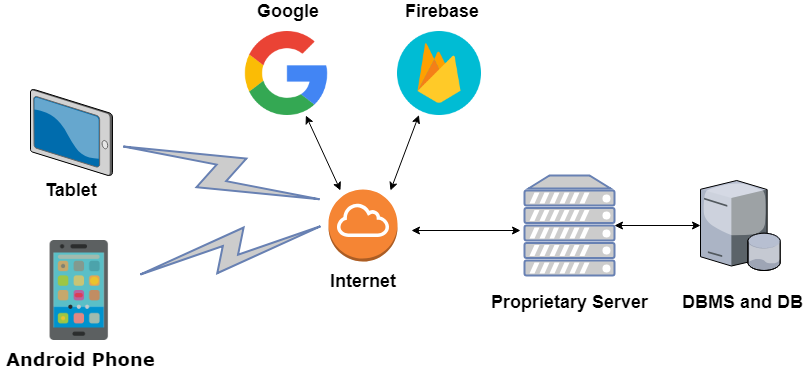
\includegraphics[scale=0.5]{Images/Diagrams/High_level_System_Architecture}
	\caption{High level system architecture}
\end{figure}

\newpage
\mysubsection{High Level Component View}
The system is divided in three main layers: Presentation Layer, Business Layer and Data Layer. The presentation layer is both mobile and tablet application. For both we have a very thin client with the main aim of performing requests to the application server in the Business layer and receives the demanded information to manage and show locally.

\vspace*{0cm}
\begin{figure}[H]
	\centering
	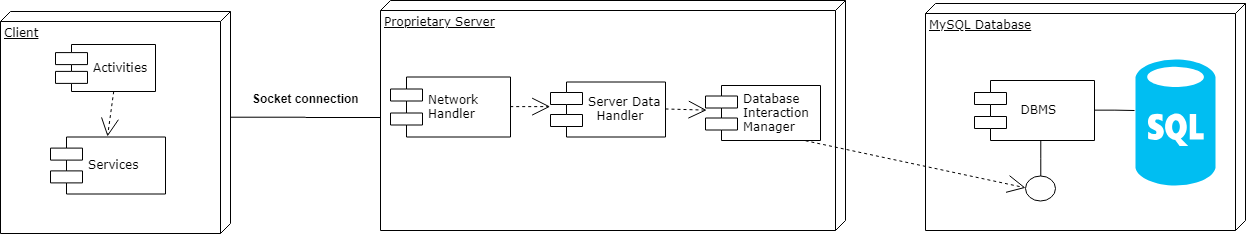
\includegraphics[scale=0.35]{Images/Diagrams/Component_diagram}
	\caption{Component View}
\end{figure}

\mysubsubsection{Client-side Application}
In this section we are going to illustrate the general architecture of our client application. The EasyLib app can be fairly considered a thin client. In fact, the most application logic is kept in the server-side. The biggest part of the logic implemented in the client is devoted to front-end purposed, that is receiving the packaged data from the server and manipulate them in order have the most intuitive and pleasant possible screen view.\\ 
In order to accomplish efficiently the communication task, the client exploits two different android services: 

\begin{itemize}
\item \emph{Connection service:}it manages the communication with the server. It opens a socket connection and keep it alive in order to send and receive messages in any moment and in an asynchronous fashion.
\item \emph{Check connection service:}It constantly checks if there is internet connection available and if is not the case makes the user aware of this forbidding any dangerous actions that could lead to a misbehaviour of the app.
\end{itemize}

As in the server side, we implemented a system to decode the messages received from the server. Here the task was heavier than the application server homologous due to some Android constraints. In fact the messages have to be passed through two different classes before reaching the application context and be manipulated to modify the view. The service thread is in charge of this massage handling. First of all the message received is used as key in a functional HashMap to trigger the correspondent method that receive the expected object from the input socket channel, wrap it in a bundle and pass it to the next class. Here another functional map allows to call the correct method and send the object along with its related message to current application context where a Broadcast receiver component is listening for incoming inputs.

\mysubsubsection{Server-side Application}
\mysubsubsection{Application Server}
As said in the previous paragraphs, EasyLib is an application that allows the user to interface with several libraries. It does so by centralizing all the libraries data inside a server that can manage multiple clients with different access privileges, that is libraries’ users and librarians, simultaneously. The clients establish a socket connection with the server from their devices and, previous authentication, it manages many kinds of stateless requests. \\
Our application server is divided in three parts: socket connection layer, request decoding layer and database manager.

\begin{itemize}
\item \emph{Socket connection layer:}this layer is always listening for new connection requests. When a new client claims to log in or register to EasyLib, the connection layer grab its request creating a new socket connection. After that the TCP connection has been established, all the communications pass through this one and the messages delivered to the subsequent component.
\item \emph{Request decoding layerr:}this layer implemented in the Java class called ServerDataHandler, receives the request grabbed by the connection layer and decodes it in order to trigger the functions to produce the requested answer on the DatabaseManager class and take back their output. The decoding of the requests has been made using a functional Hash Map that has as key a string and as value a function reference that is triggered when the correspondent string is received from the client.
\item \emph{Database manager:}this final layer is the core of the system business logic. It receives the directive from the previous layer, produces SQL statement and send them to the DBMS to retrieve the requested data. Then, it manipulates and format the data before sending them back to the client through the Socket connection layer.
\end{itemize}


\mysubsection{External Services}
EasyLib exploits some external services to accomplish its main tasks.

\begin{itemize}
\item \emph{Google sign in:}we use google sign in API to allow the user to identify himself in our system with his google credentials.
\item \emph{Firebase Cloud Messaging: } we use Firebase Cloud Messaging system to manage the notification that our server needs to send to the user.
\item \emph{Google Books API:}we use google books API to fill the books schema of the libraries’ database.
\end{itemize}

\mysubsection{Data Layer}
The data layer is composed by a multi-table MySQL database that allow to persistently store all the data that the application need to provide its services. In the current moment it is composed by three schemas: the proprietary\_db, library\_1 and library\_2. The EasyLib system is designed to be scalable and include any number of libraries that want to join our project. The only constraint that they have to follow is to homologate their database to our scheme, in order to provide the access to their information to the application. 

\mysubsubsection{Database structure}
The Database is composed by two main schemas: proprietary\_db and library\_x. The former contains the information about the users and librarians’ identity, the libraries’ info needed to distinguish them, the book read by all the users and their favourite libraries.\\
The latter contains all the information strictly related with a single library. The x stands for an integer and represents the id related with the library. It contains information about the books, the news, the events and their participants, the books reserved and the queue for them and the ratings related to the book read in that library.\\
Some of the tables in these schemas contains triggers used to maintain the consistence of the data and to build more meaningful information to show to the final user. 


\vspace*{0cm}
\begin{figure}[H]
	\centering
	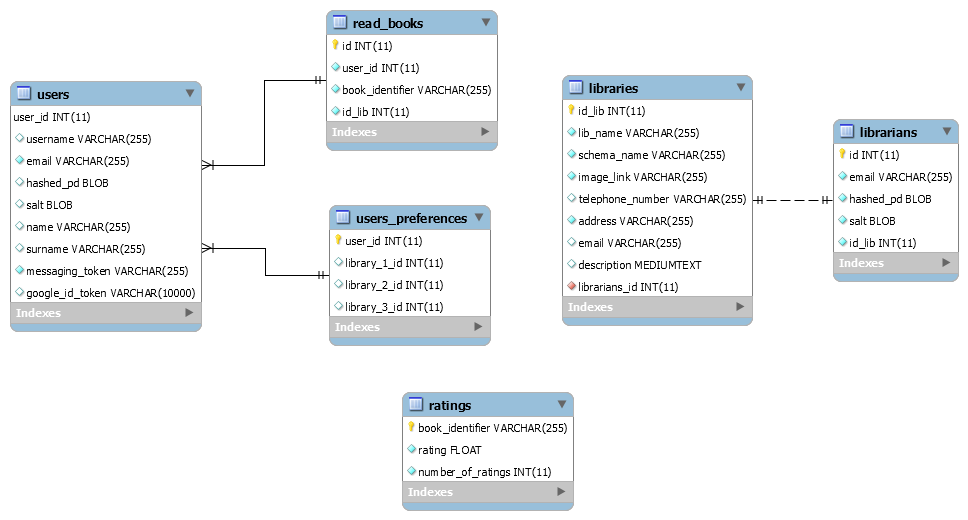
\includegraphics[scale=0.50]{Images/Diagrams/proprietary_db_UML}
	\caption{Proprietary database}
\end{figure}

\vspace*{0cm}
\begin{figure}[H]
	\centering
	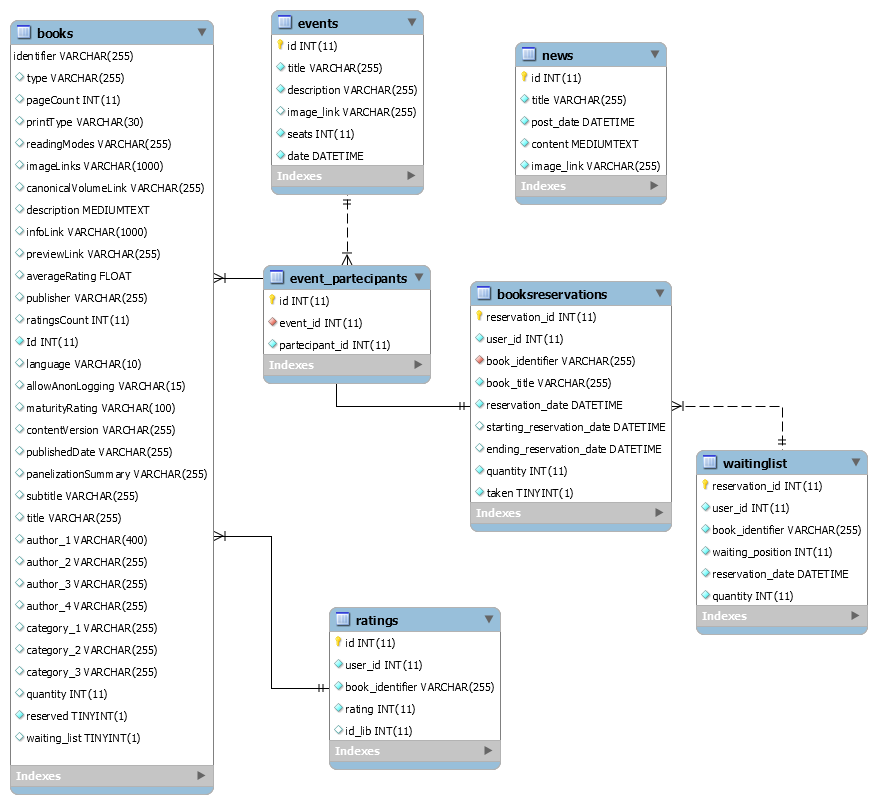
\includegraphics[scale=0.50]{Images/Diagrams/library_db_UML}
	\caption{Library database}
\end{figure}

\mysubsubsection{Triggers}
In order to maintain the data consistency after that users perform state changing operations, we have implemented 9 triggers distributed between the various schemas and tables. We list all of them below along with the description of their behaviour.

\mysubsubsection{Library schema}

\begin{tabular}[H]{p{4cm}|p{4cm}|p{4cm}}
	\textbf{Trigger name} & \textbf{Table name} & \textbf{When} \\
	\hline
	\rule{0pt}{4ex} On\_insert\_rating  & ratings & after insert \\
	\hline
\end{tabular}
\vspace{0.8cm}
\\
It computes the updated average rating of a book including the inserted rating and store it in the table ratings of the proprietary\_db if it does not exist or update a currently existing record.

\vspace{0.8cm}
\begin{tabular}[H]{p{4cm}|p{4cm}|p{4cm}}
	\textbf{Trigger name} & \textbf{Table name} & \textbf{When} \\
	\hline
	\rule{0pt}{4ex} update\_count\_on
	\_delivering  & booksreservations & after delete \\
	\hline
\end{tabular}
 \vspace{0.8cm}\\
It updates the count of available copies for a book in books table in library\_x schema after that one of them has been delivered. If the current available number of copy result to be zero after the action, the Boolean reserved is set to true.


\vspace{0.8cm}
\begin{tabular}[H]{p{4cm}|p{4cm}|p{4cm}}
	\textbf{Trigger name} & \textbf{Table name} & \textbf{When} \\
	\hline
	\rule{0pt}{4ex} waiting\_list\_flowing  & booksreservations & after delete \\
	\hline
\end{tabular}
 \vspace{0.8cm}\\
It updates the position of the users in line of the book with the identifier equal to that one of the record deleted in the booksreservations table and remove the first waiting user for the book since it has to be inserted in the bookreservations table.

\vspace{0.8cm}
\begin{tabular}[H]{p{4cm}|p{4cm}|p{4cm}}
	\textbf{Trigger name} & \textbf{Table name} & \textbf{When} \\
	\hline
	\rule{0pt}{4ex} update\_on\_reservation  & booksreservations & after insert \\
	\hline
\end{tabular}
\vspace{0.8cm}
\\

It updates the count of available copies for a book in books table in library\_x schema after that one of them has been returned to the librarian of library x.

\vspace{0.8cm}
\begin{tabular}[H]{p{4cm}|p{4cm}|p{4cm}}
	\textbf{Trigger name} & \textbf{Table name} & \textbf{When} \\
	\hline
	\rule{0pt}{4ex} update\_on\_reservation  & booksreservations & after insert \\
	\hline
\end{tabular}
\vspace{0.8cm}
\\
It updates the count of available copies for a book in books table in library\_x schema after that one of them has been returned to the librarian of library x.

\vspace{0.8cm}
\begin{tabular}[H]{p{4cm}|p{4cm}|p{4cm}}
	\textbf{Trigger name} & \textbf{Table name} & \textbf{When} \\
	\hline
	\rule{0pt}{4ex} update\_available\_
	seats\_ins  & event\_partecipants & after insert \\
	\hline
\end{tabular}
\vspace{0.8cm}
\\
It updates the count of available seats for an event after a registration for it has been performed.

\vspace{0.8cm}
\begin{tabular}[H]{p{4cm}|p{4cm}|p{4cm}}
	\textbf{Trigger name} & \textbf{Table name} & \textbf{When} \\
	\hline
	\rule{0pt}{4ex} update\_available\_
	seats\_del  & event\_partecipants & after delete \\
	\hline
\end{tabular}
\vspace{0.8cm}
\\
It updates the count of available seats for an event after that a registration for it has been removed.

\vspace{0.8cm}
\begin{tabular}[H]{p{4cm}|p{4cm}|p{4cm}}
	\textbf{Trigger name} & \textbf{Table name} & \textbf{When} \\
	\hline
	\rule{0pt}{4ex} on\_insert\_waiting\_
	person  & waitinglist & before insert \\
	\hline
\end{tabular}
\vspace{0.8cm}
\\
It sets the position in the waiting list of the new user inserted in the table for a book.

\vspace{0.8cm}
\begin{tabular}[H]{p{4cm}|p{4cm}|p{4cm}}
	\textbf{Trigger name} & \textbf{Table name} & \textbf{When} \\
	\hline
	\rule{0pt}{4ex} update\_waitinglist\_
	position  & waitinglist & after delete \\
	\hline
\end{tabular}
\vspace{0.8cm}
\\
It updates the position of the users in line for a book after that a user in line has deleted is presence in the queue.

\mysubsubsection{Proprietary schema}
\begin{tabular}[H]{p{4cm}|p{4cm}|p{4cm}}
	\textbf{Trigger name} & \textbf{Table name} & \textbf{When} \\
	\hline
	\rule{0pt}{4ex} on\_insert\_rating
	\_propDB  & ratings & after insert \\
	\hline
\end{tabular}
\vspace{0.4cm}
\\
It updates the average rating for the considered book in all the libraries of the system.
\vspace{0.4cm}



\mysubsubsection{Internal customized data structures}
In order to make the communication easier and the data transmission between the clients and the application server manageable, we have created few serializable data structures that are sent over the internet. They are 13 java classes designed with the purpose of containing all the information that server and clients need to exchange such as: books information, reservation details, events schedule, etc. 

\mysubsection{Deployment View}
Here we provide a deployment strategy for our system.

\vspace*{0cm}
\begin{figure}[H]
	\centering
	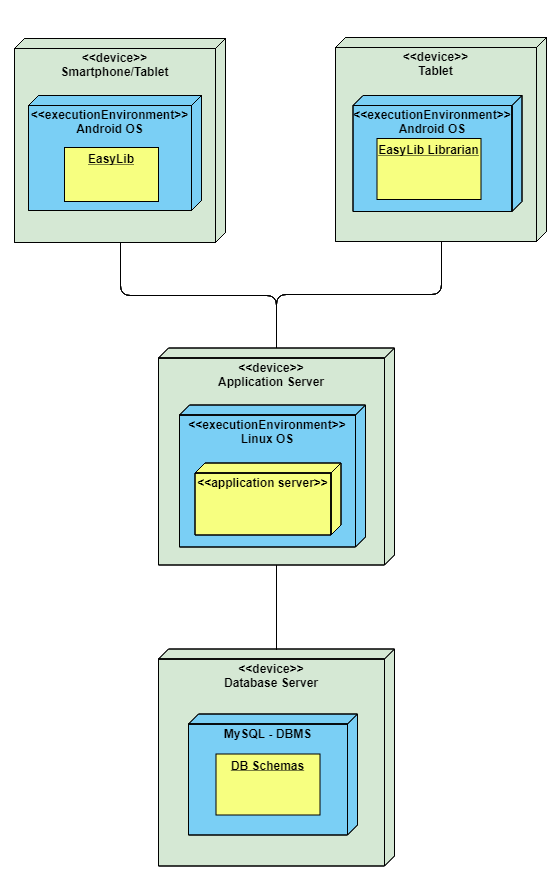
\includegraphics[scale=0.55]{Images/Diagrams/Deployment_view_EasyLib}
	\caption{Deployment view EasyLib}
\end{figure}
\mysubsection{Non-Functional Requirements}
Here we state some non functional requirements that our system must respect during the execution.

\begin{itemize}
\item \emph{Performance:} The system must be able to respond to a consistent number of user requests simultaneously. All the data requested by the users and the needed computations must respectively retrieved and performed as soon as possible and as efficiently as possible.

\item \emph{Reliability:} The system must guarantee a 24/7 service. The information must be stored in proprietary Database in order to be always available to the user when required.
\item \emph{Scalability:} The system must ensure a high level of scalability, since new libraries can join the system in any moment enlarging EasyLib supply.
\item \emph{Security:} All users’ passwords are encrypted using a hash function with salt. In this way the attacker cannot see the plain text password and steal sensitive information.

\item \emph{Accuracy:} The data retrieved by the application has to be accurate and up-to-date in a real-time fashion.
\end{itemize}
	\newpage
	\vspace*{-5mm}
\mysection{User Interface Design}

\color{red} general description + made 2 types of screen resolution normal + xlarge
\color{black}


\mysubsection{Special Android Features used for UI}


\mysubsection{Functions Flow}
	\newpage
	\vspace*{-5mm}
\mysection{Runtime View}
In this section we will see some Runtime Views in order to see how the components interact according to specific requests.\par
For the server-side we have taken into consideration the high-level Application Server only, without identifying the specific components of it. We also separate it from the DB, cause they are in 2 different machines.

\mysubsection{EasyLib}
\vspace*{0.5cm}

\mysubsubsection{QR-Code Scan + Book Reservation}
This Runtime View shows the different steps needed to find book information through QR-code scan and reserve it.\par
We have to make an assumption : in the following diagram we reported only the most meaningful calls needed to achieve the goal.\par
So starting from the Main Activity the User has to tap the “QR scan” icon on the bottom NavBar and the EasyLib app will open the “QR Scan Activity”. Thanks to the camera of the smartphone or tablet the QR-image is captured and an identifier is returned. This one is the book identifier and is sent to the server (and so the DB) to get back the information. The “Book Activity” is started and book information are set in the layout.\par
In order to let the user reserve the book, the app gets from the server (and so the DB) a list of libraries where it’s available. They are next passed to the BookActivityAdapter that creates the single items of the recyclerView placed under the book information.
\newpage
\vspace*{0cm}
\begin{figure}[H]
	\centering
	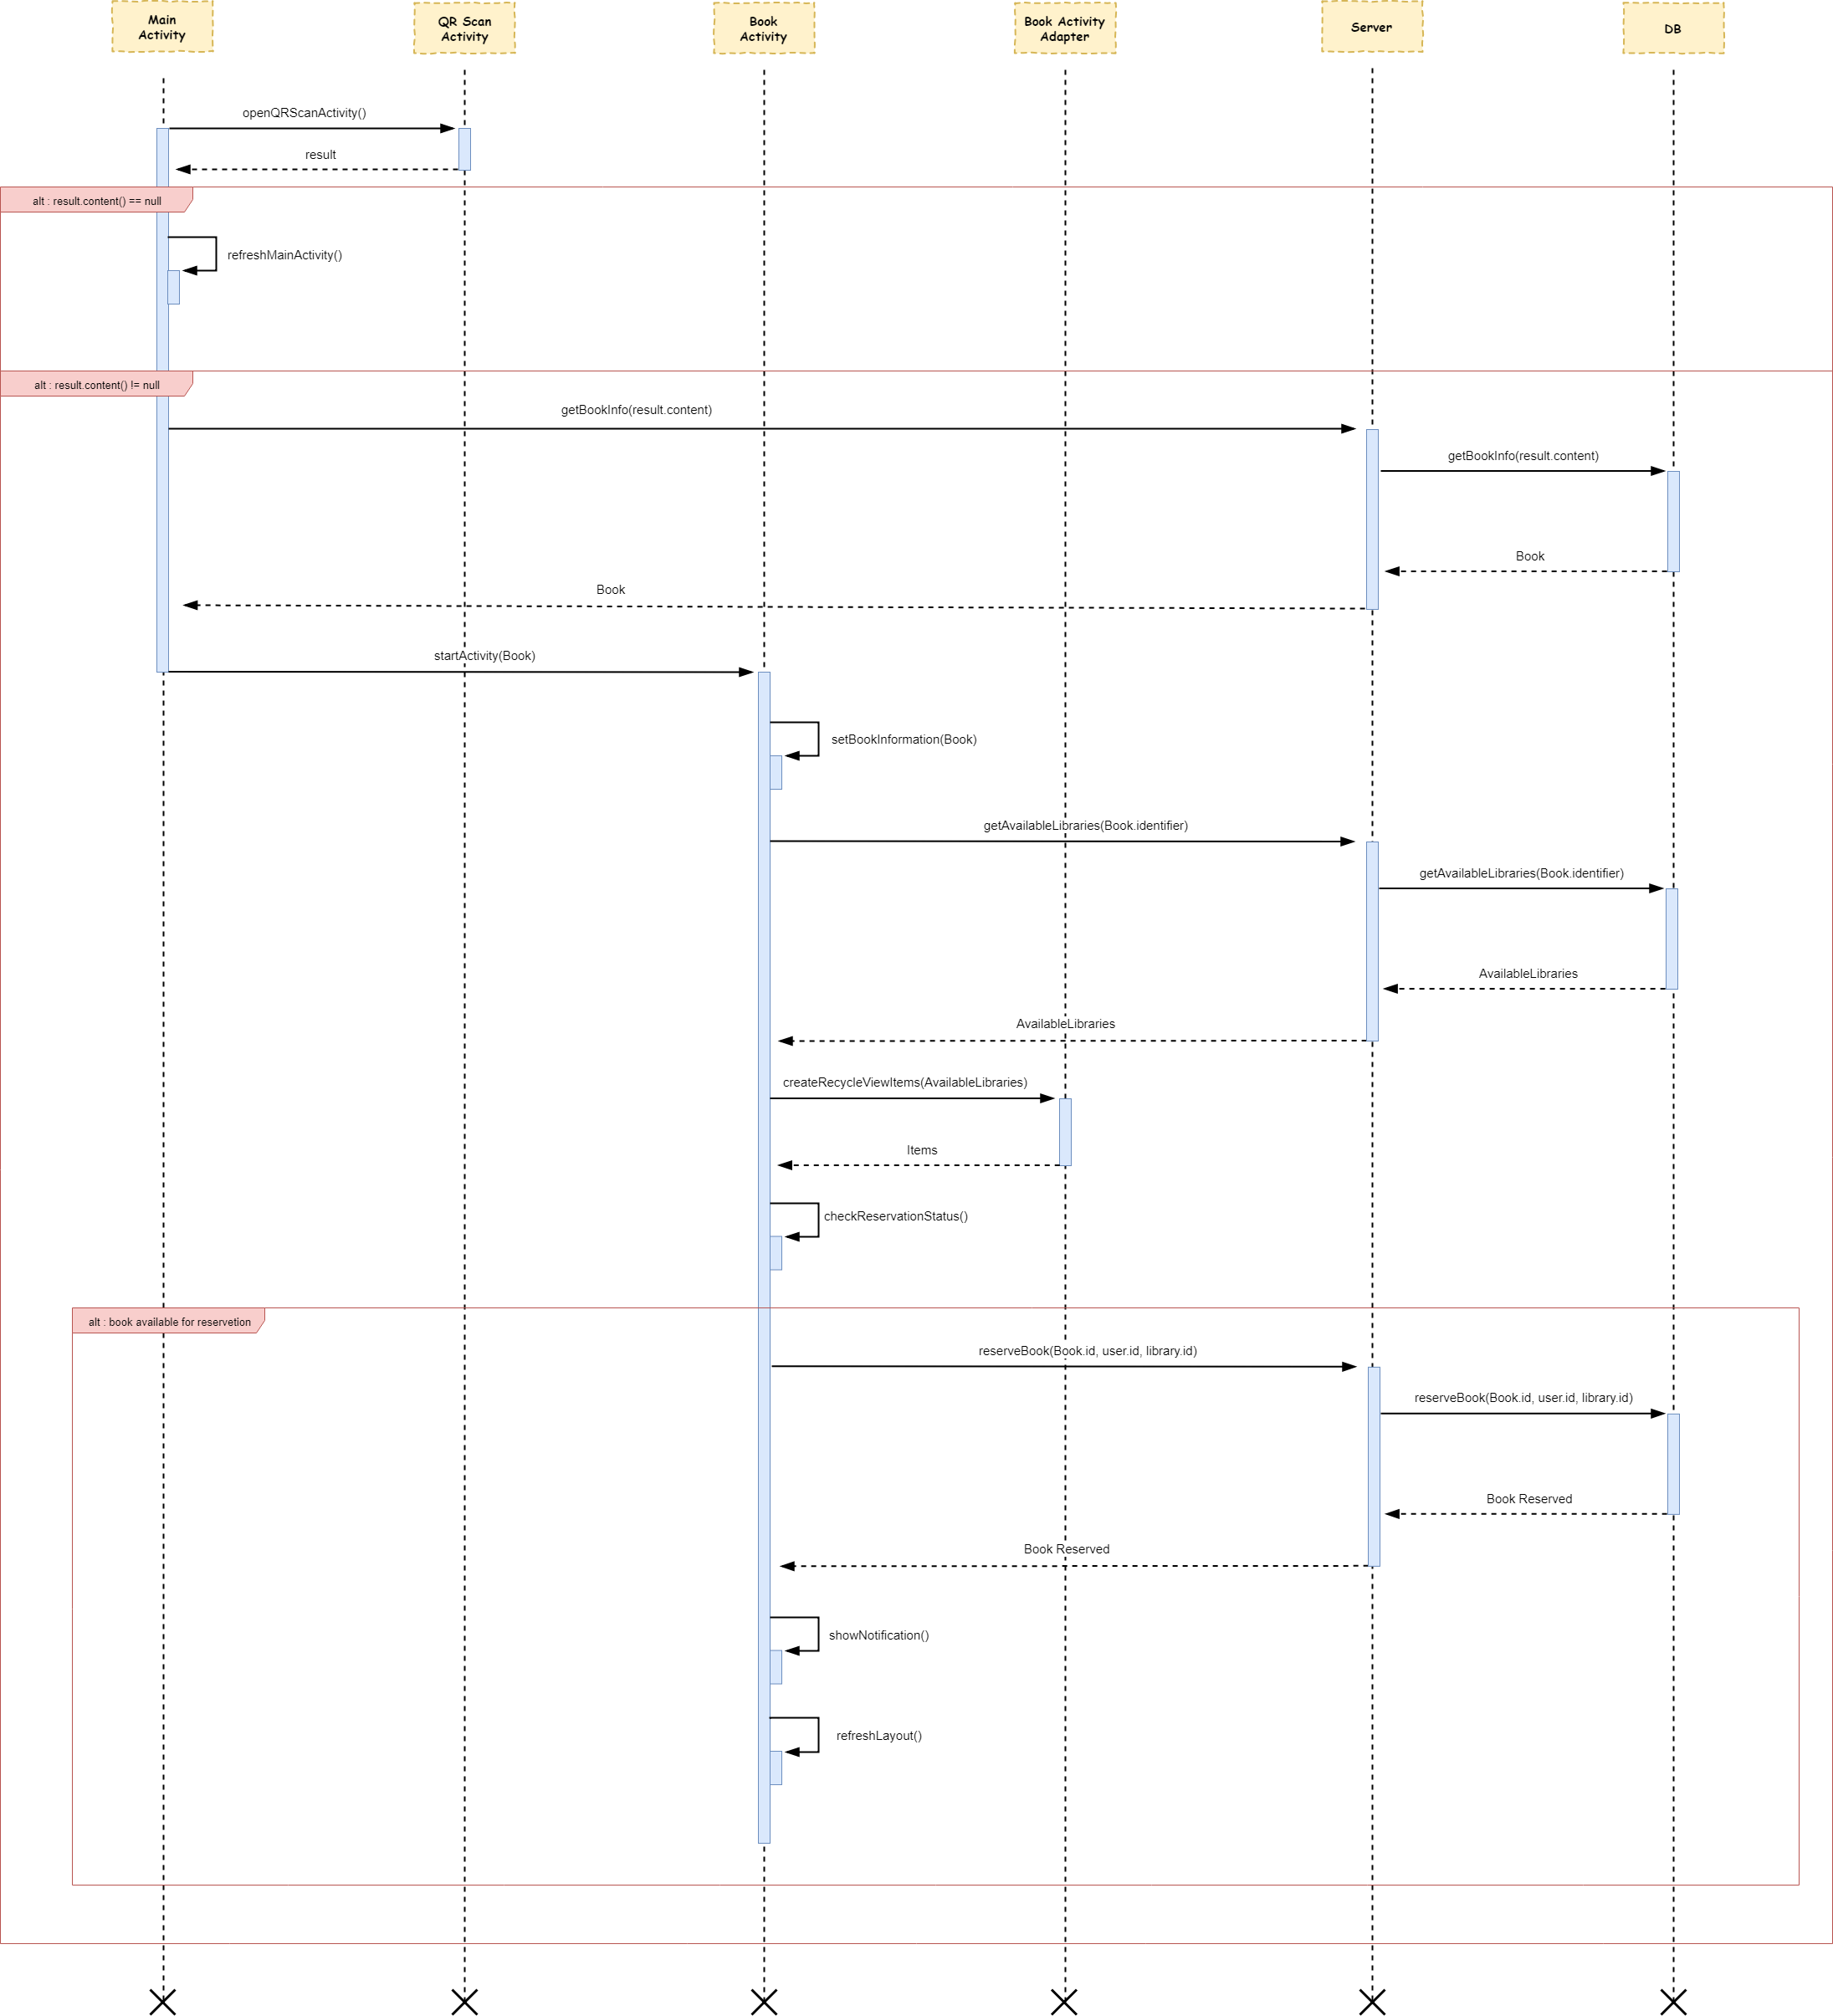
\includegraphics[scale=0.21]{Images/Runtime/user_qrcode_reserve}
	\caption{QR-Code Scan + Book Reservation - Runtime View}
\end{figure}

\newpage
\vspace*{0cm}
\mysubsubsection{Rate Book}
This Runtime View shows the different steps needed to rate a book.
We have to make some assumption :
\begin{itemize}
	\setlength{\leftskip}{0.5cm}
	\item In the following diagram we reported only the most meaningful calls needed to achieve the goal.
	\item The book can be rated only if it was previously reserved and read through EasyLib app.
\end{itemize}
So starting from the Main Activity the User has to tap the “Profile” icon on the bottom NavBar and the EasyLib app will ask the server for User information sending his user identifier. Once data are back, "Main Activity" sets the "Profile Fragment" in the Main Frame.\par
Next the app asks the server for the read books and shows them in the "Read Books Activity" that contains a recyclerView. The user can select the wanted book and open it in the "Book Activity". When it starts the book information, passed with an Intent, are set in the layout and a check is made in order to see if the it's already rated by the user or not. In case it's not, an EditText is showed and the user can fill it with a rate from 0 to 10.
\newpage
\vspace*{0cm}
\begin{figure}[H]
	\centering
	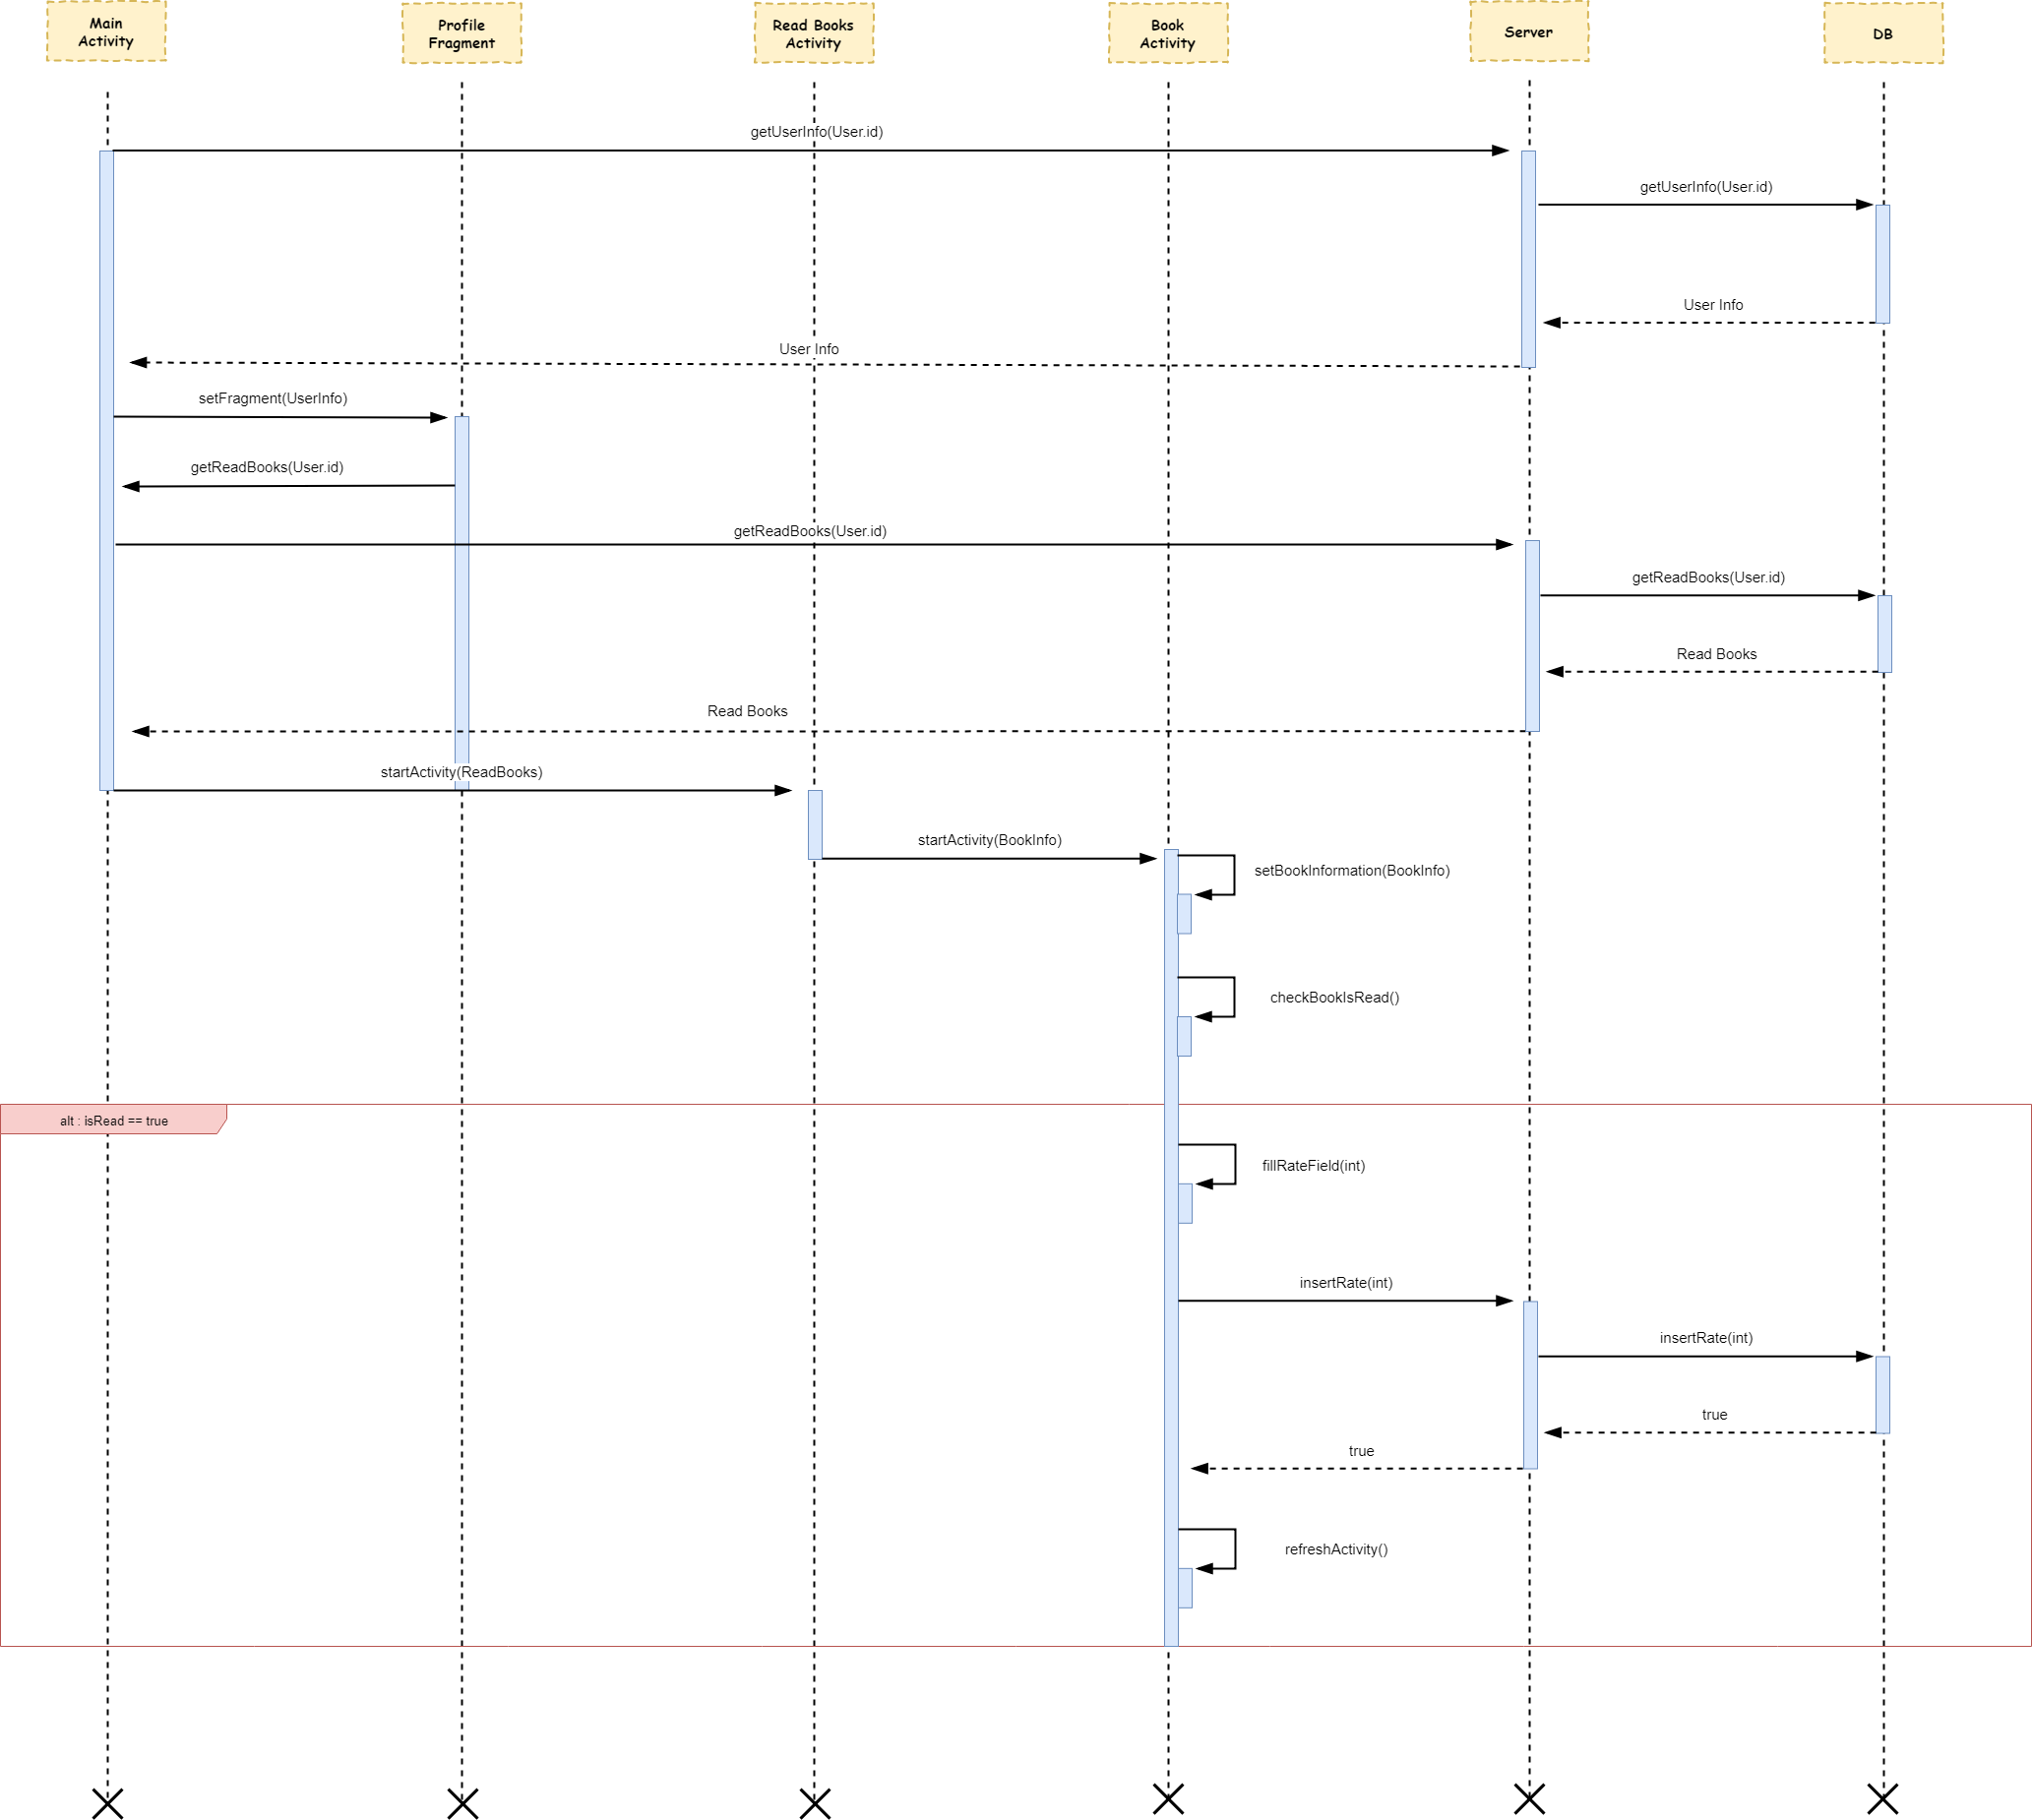
\includegraphics[scale=0.22]{Images/Runtime/rate_book}
	\caption{Rate Book - Runtime View}
\end{figure}

\newpage
\vspace*{0cm}
\mysubsubsection{Event - Reserve Seat}
This Runtime View shows the different steps needed to reserve a seat. \par
We have to make an assumption : in the following diagram we reported only the most meaningful calls needed to achieve the goal. \par
So starting from the Main Activity the User can tap the “All Libraries” button and the EasyLib app will ask the server (and so the DB) to get the list of all of them. On return a new activity is started where thanks to a RecyclerView the list of all the libraries is displayed. \par
The user can next select the Library that he wants and like the libraries list, the information about this one are asked to the server and next displayed in the Book Activity. In this activity are displayed also the “library contents” (news, events and books), so user can select an event and automatically the EventActivity is opened and shown.\par
The app will check if there are available seats and if the user has already joined the event (in the diagram is called “checkEventStatus()”). So if there free seats and the event is not already joined then the “Reserve Seat” button is shown and the User can reserve a seat.
\newpage
\vspace*{0cm}
\begin{figure}[H]
	\centering
	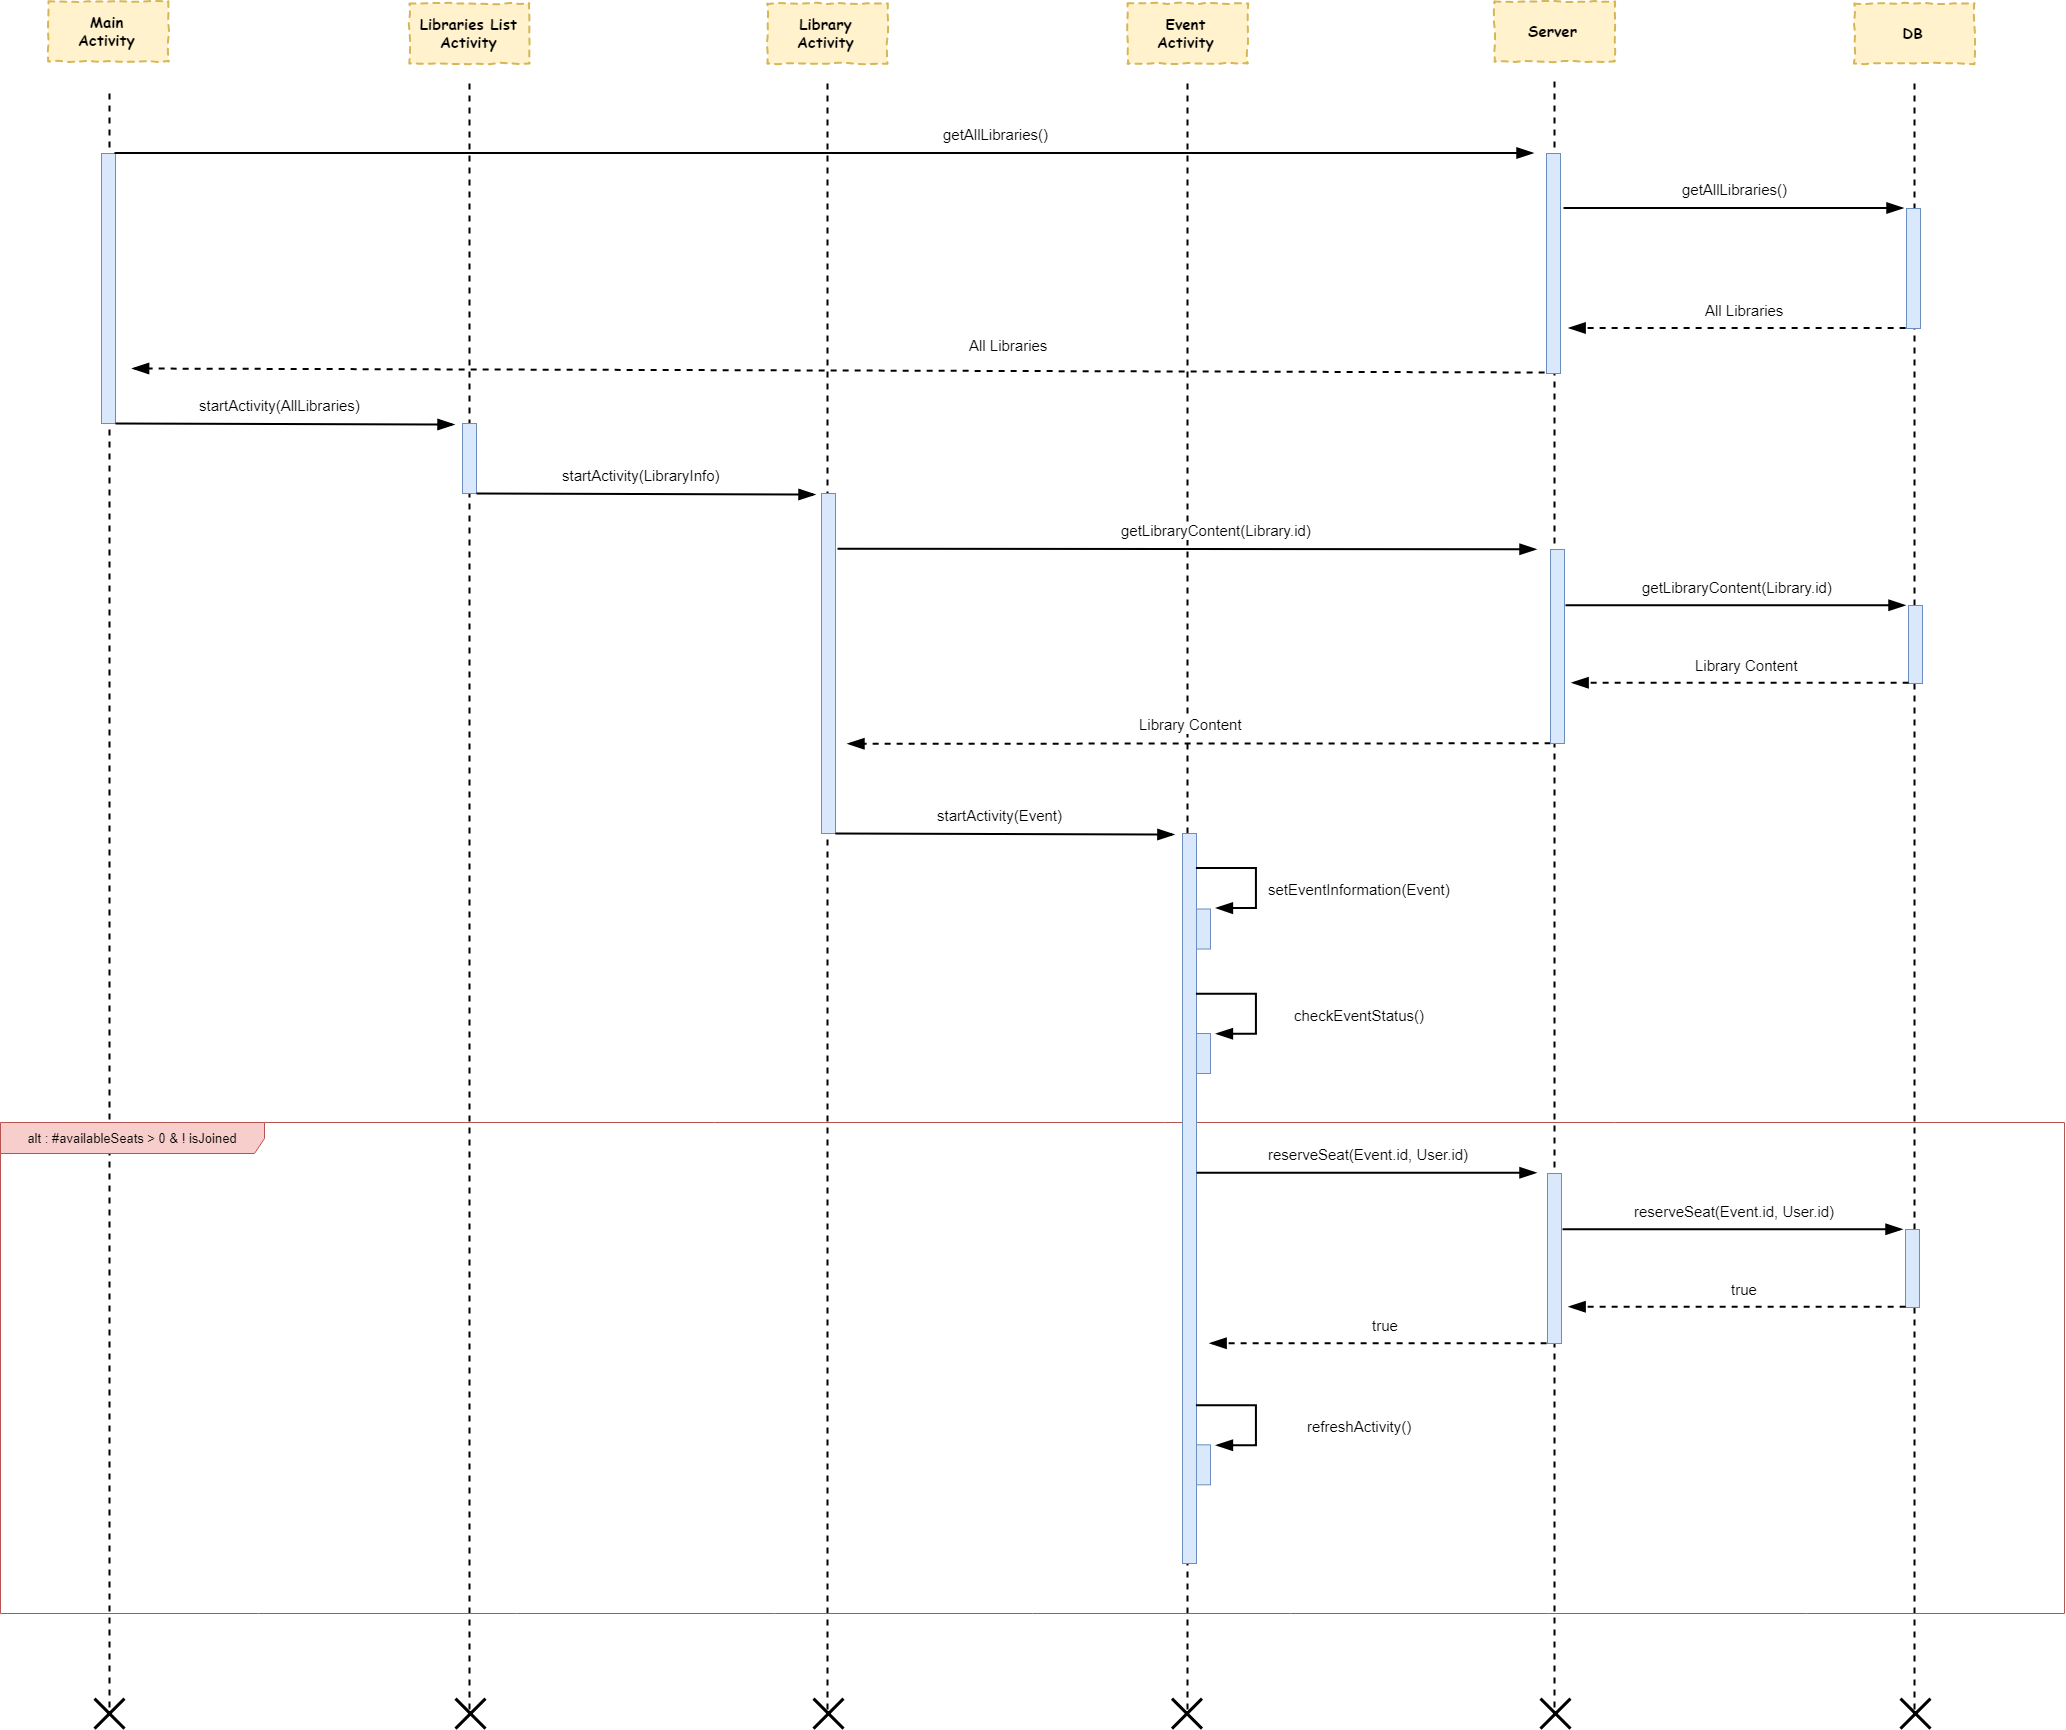
\includegraphics[scale=0.22]{Images/Runtime/event_reserve_seat}
	\caption{Event Reserve Seat - Runtime View}
\end{figure}

\newpage
\vspace*{0cm}
\mysubsection{EasyLib - Librarian}
\vspace*{0.5cm}

\mysubsubsection{QR-Code Scan + Book Returned}
This Runtime View shows the different steps needed to find book information through QR-code scan and communicate to the serve (and so the DB) that the book is returned.\par
We have to make an assumption : in the following diagram we reported only the most meaningful calls needed to achieve the goal.\par
So starting from the "Library Activity" the librarian has to tap the Floating Button with the QR-code icon that allows the app to open the "QR Scan Activity". As in the previous runtime, the qr-code is analyzed and the identifier returned is used to get from the server (and so the DB) the information of that specific book. The "Book Activity" is then opened and data are set in the layout.\par
The app has next to get all the reservations and pass the ArrayList to an Adapter that generates the single items of the recyclerView placed under the book layout.\par
At the end the librarian as to find the reservation that has the user id and tap the "Returned" button.
\newpage
\vspace*{0cm}
\begin{figure}[H]
	\centering
	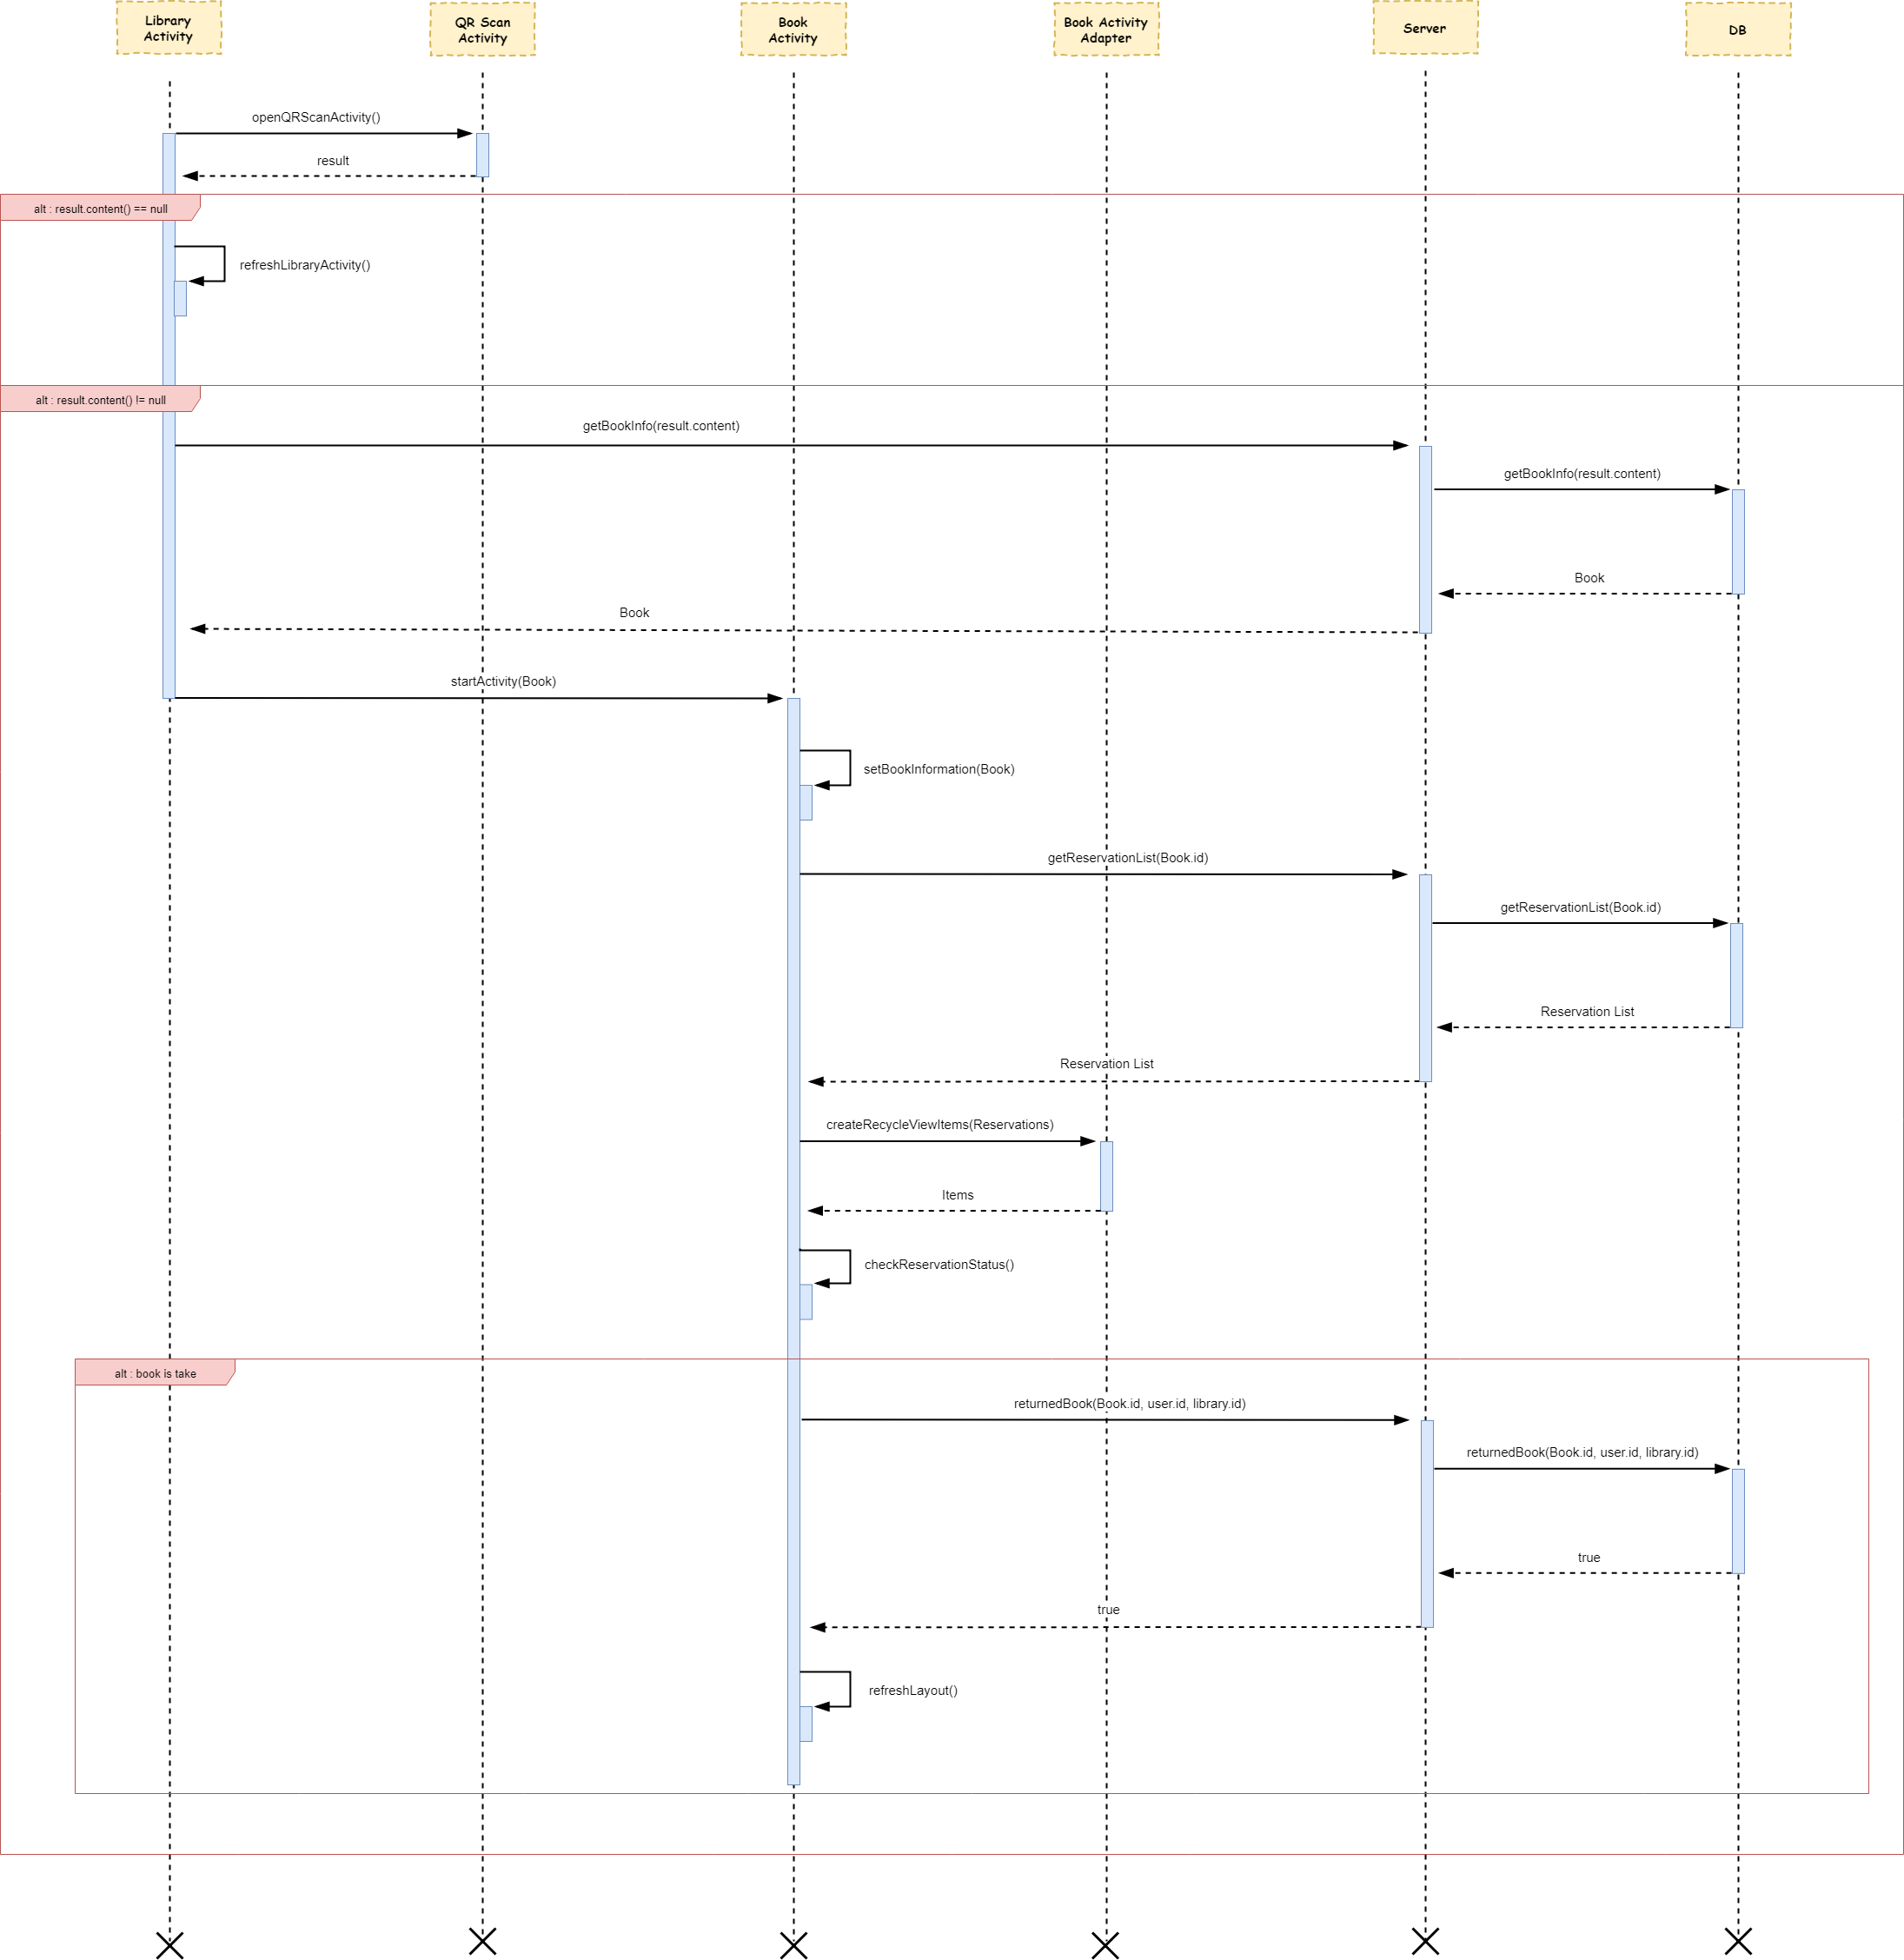
\includegraphics[scale=0.21]{Images/Runtime/librarian_qrcode_returned}
	\caption{QR-Code Scan + Book Returned - Runtime View}
\end{figure}
	\newpage
	\vspace*{-5mm}
\mysection{Implementation, Integration \& Test Plan}
In this section we will show the plan we have projected for implementing EasyLib. We will describe the strategy for the processes chosen for approaching the project and the structure of our team, how it is divided and the tasks that each part has to accomplish. After we will state how each team’s part has to interact with the others and the span of time of these interactions. Finally, we will supply a list of possible risks, the probability of their presence, their impact and a possible strategy to deal with them.

\mysubsection{Strategy adopted}
To give a quality assurance of the project and to be sure that the final product we have followed an Agile planning process. It consists in a first initiating part in which we have stated an overall plan application that we have implemented. We have defined the EasyLib’s requirements, discussed and stated the flow of each interaction and the specific technology to use. 
After this part, we followed the well know agility’s cycle, composed by the subsequent phases: Executing, monitoring and Controlling, Closing and Planning. Every cycle round has as input a specific process to accomplish, that is divided between the various team’s parts. After the execution of all the tasks in a precise given timeframe, the work were checked by all the parts. When the discussion on the work done has been terminated and an agreement has been reached, another planning phase containing also the corrections agreed. This cycle has been repeated until the end of the project.

\mysubsection{Team Structure}
Our team is composed by two Computer engineers with complementary competences and that have dealt with different tasks throughout the development process. The main tasks performed are that one listed and commented right below.

\begin{itemize}
\item \emph{Client Front-End development:}this role required the full understanding of the android components related to the visualization part, the high level of image-editing software in order to produce the aimed layout and the management of the application server requests and the arrangement of the information contained in the responses to produce the whished view result. 

\item \emph{Client Back-End and Application Server development:} this role required a deep knowledge of how to build asynchronous socket multi-client network infrastructure, a good understanding in multi-table MySQL databases management, including SQL statement and trigger implementation. Nonetheless, this team component has dealt with the Android services and their communication with the application server and the main thread of the app.
\end{itemize}

\mysubsection{Implementation process}
The work has been divided in three milestones. In these spans of time the team members were required to complete the tasks that have been established in the previous planning phase. Every week a meeting to discuss about the progresses were attended and new agreement finalized to proceed at the same speed were taken. If a team’s part terminated his tasks before the milestone’s day, it usually anticipated the work programmed for the subsequent milestone but remaining ready for eventually applying changes or corrections on the software already implemented. After each milestone, some days were employed for integrating front-end and back-end part to have always a working prototype. \\
At the end of the implementation process the team has performed a Unit testing and functional testing campaign, in order to assure that all the functionalities worked correctly. Also a User acceptance test have been carried on, involving a restrict group of people which gave back feedback on their user experience that drove the developing process.



\end{document}